\documentclass{beamer}
% September 2014 
% Author: Dr Rachid Hourizi and Dr. Michael Wright 
% Department of Computer Science, University of Bath
\usepackage{listings}
\usetheme{Boadilla} 
\usepackage{fixltx2e}
\usepackage{hyperref}
\lstset{language=Java,,
	basicstyle=\ttfamily\small,
           keywordstyle=\color{blue}\ttfamily,
           stringstyle=\color{red}\ttfamily,
           commentstyle=\color{gray}\ttfamily,
          breaklines=true}

\begin{document}

\AtBeginSection[]{
  \begin{frame}
  \vfill
  \centering
  \begin{beamercolorbox}[sep=8pt,center,shadow=true,rounded=true]{title}
    \usebeamerfont{title}\insertsectionhead\par%
  \end{beamercolorbox}
  \vfill
  \end{frame}
}

\title{CM 10227: Lecture 8}
\author{Dr Rachid Hourizi and Dr Michael Wright}
\date{\today}
\frame{\titlepage}

\begin{frame} 
\begin{center}
\textbf{Resources}
\end{center}
\begin{itemize}
\item More help with this course
\begin{itemize}
\item Moodle
\item E-mail - programming1@lists.bath.ac.uk
\end{itemize}
\item Online C and Java IDE
\begin{itemize}
\item https://www.codechef.com/ide
\item Remember to select Java from the drop down menu.
\end{itemize}
\item Books
\begin{itemize}
\item Java by Dissection (Free pdf online)
\item The Java Tutorial (https://docs.oracle.com/javase/tutorial/)
\end{itemize}
\end{itemize}
\end{frame}

\begin{frame} 
\begin{center}
\textbf{Resources}
\end{center}
\begin{itemize}
\item The places that you can get additional support if you are finding the pace of the course a little fast now include
\begin{itemize}
\item A labs (Continued from week 1)
\item B labs 
\item ... Wednesday 11:15-13:05 EB0.7
\item ... Fridays 17:15 to 19:15 in CB 5.13)
\item The Drop in Session 
\item ... booked 20 min appointments
\item ... Friday 11.15-13.05 1E 3.9
\item PAL sessions (Mondays 14:15 to 15:05 1E 3.9)
\end{itemize}
\end{itemize}
\end{frame}

% *** CONTENT ***

\begin{frame}
\begin{center}
\textbf{Last Week}
\end{center} 
\begin{itemize}
\item Recap on Classes and Objects
\bigskip
\item Inheritance
\item Polymorphism
\end{itemize}
\end{frame}

\begin{frame}
\begin{center}
\textbf{This Week}
\end{center} 
\begin{itemize}
\item Interfaces 
\item Abstract Classes
\end{itemize}
\end{frame}

\begin{frame}
\begin{center}
\textbf{Recap: Inheritance and Polymorphism}
\end{center}
\end{frame}

\begin{frame}
\begin{itemize}
\item Last week we looked at inheritance
\end{itemize}
\end{frame}

\begin{frame}[fragile]
\begin{center}
\item Database Of Multimedia Entertainment 
\end{center}
\begin{block}{}
\begin{lstlisting}
public  class  Item{
    private  String  title ;
    private  int  playingTime ;
    private  boolean  gotIt ;
    private  String  comment;
    
    // constructors  and  methods  omitted ...
}

public  class  MusicFile  extends  Item{
    private  String  artist;
    private  int  numberOfTracks;
    // constructors  and  methods  omitted
}
\end{lstlisting}
\end{block}
\end{frame}

\begin{frame}[fragile]
\begin{center}
\item Database Of Multimedia Entertainment (... of my youth)
\end{center}
\begin{block}{}
\begin{lstlisting}
public  class  Item{
    private  String  title ;
    private  int  playingTime ;
    private  boolean  gotIt ;
    private  String  comment;
    
    // constructors  and  methods  omitted ...
}

public  class  CD  extends  Item{
    private  String  artist;
    private  int  numberOfTracks;
    // constructors  and  methods  omitted
}
\end{lstlisting}
\end{block}
\end{frame}

\begin{frame}
\begin{itemize}
\item Looked at the concept of overridding methods 
\item i.e. extending or rewriting methods in subclasses when they already exist in superclasses
\end{itemize}
\end{frame}

\begin{frame}
\begin{center}
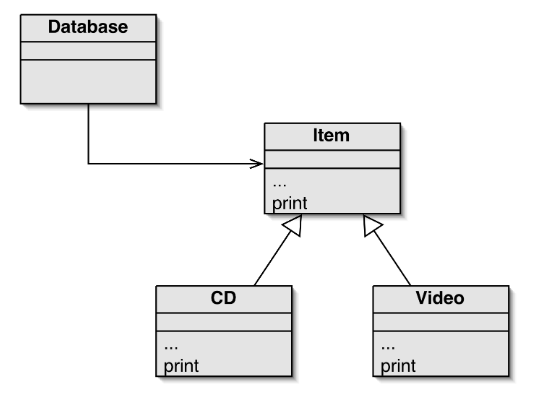
\includegraphics[height=7cm, keepaspectratio]{images/poly3}
\end{center}
\end{frame}

\begin{frame}
\begin{center}
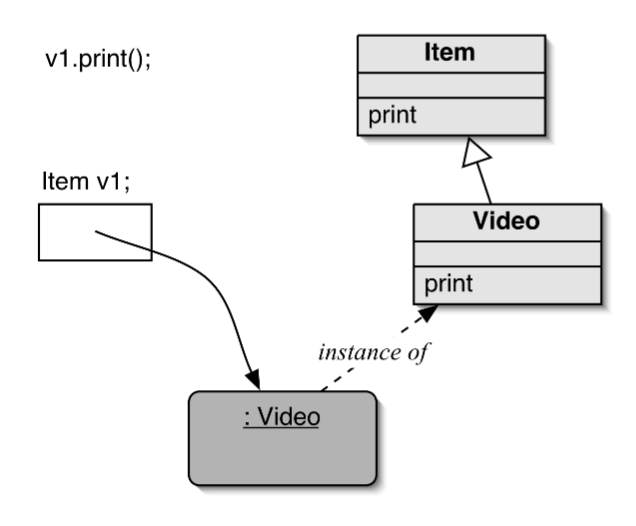
\includegraphics[height=7cm, keepaspectratio]{images/poly5}
\end{center}
\end{frame}

\begin{frame}
\begin{center}
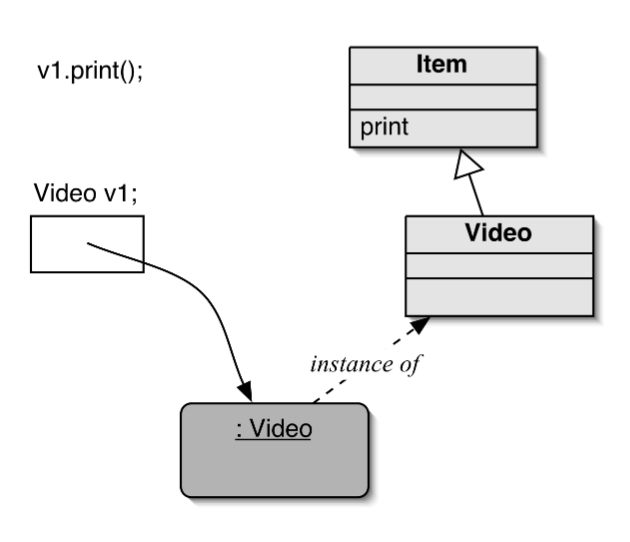
\includegraphics[height=7cm, keepaspectratio]{images/poly6}
\end{center}
\end{frame}

\begin{frame}
\begin{center}
\textbf{Question}
\end{center} 
\begin{itemize}
\item Does it make sense in out Database of Multimedia Entertainment to be able to instantiate Item objects?
\item i.e. is adding an Item to our database meaningful?
\end{itemize}
\end{frame}

\begin{frame}
\begin{center}
\textbf{Question}
\end{center} 
\begin{itemize}
\item Does it make sense in out Database of Multimedia Entertainment to be able to instantiate Item objects?
\item i.e. is adding an Item to our database meaningful?
\bigskip
\item Not really...
\item ... it would be better to use an Interface
\end{itemize}
\end{frame}

\begin{frame}
\begin{center}
\textbf{Interfaces}
\end{center}
\end{frame}

% *** INTERFACES ***

\begin{frame}
\begin{itemize}
\item At some point we may want an even looser relationship between superclass and subclass
\item We may want to specify a superclass in which no methods are implemented...
\item ... leaving subclasses to do all of the implementation
\end{itemize}
\end{frame}

\begin{frame}
\begin{itemize}
\item For example, we might want to describe the methods provided by all classes that can be added to our DOME
\item ... and not specify anything about the way these items are printed
\item ... i.e. we want all the implementation described elsewhere
\bigskip
\item We might specify the Item interface
\end{itemize}
\end{frame}

\begin{frame}
\begin{itemize}
\item In Java, this ``specify but implement nothing'' approach is achieved through the use of Interfaces
\item ... use the \textbf{implements} keyword in the classes we define
\end{itemize}
\end{frame}

\begin{frame}[fragile]
\begin{itemize}
\item Item interface
\end{itemize}
\begin{block}{}
\begin{lstlisting}
interface Item{   
   void print();
}

public class CD implements Item{
    private String title;
    
    public void print(){
        System.out.println(this.title);
    }
}
\end{lstlisting}
\end{block}
\end{frame}

\begin{frame}
\begin{itemize}
\item A Java interface is a specification of a type 
\item ... in the form of a type name and methods 
\item ... that does not define any implementation of methods
\bigskip
\end{itemize}
\end{frame}

\begin{frame}
\begin{itemize}
\item A Java interface...
\item ... uses \textbf{interface} instead of \textbf{class}
\item ... all methods are public (no need to mention)
\item ... all methods are abstract i.e. contains no implementation \newline (again no need to mention)
\item ... no constructors
\item ... only constant fields are allowed - \textbf{public static final}
\end{itemize}
\end{frame}

\begin{frame}
\begin{center}
\textbf{Aside : static and final}
\end{center}
\begin{itemize}
\item \textbf{static}
\bigskip 
\item means that the variable or method is shared between all instances of that class
\item it belongs to the type, not the actual objects themselves
\item e.g.  if you have a variable:  \textbf{private static int i = 0;}
\item and you increment it in one instance - \textbf{i++;} 
\item the change will be recreated in all instances
\end{itemize}
\end{frame}

\begin{frame}
\begin{center}
\textbf{Aside : static and final}
\end{center}
\begin{itemize}
\item \textbf{final}
\bigskip 
\item you cannot change the value of  final variable, method or class
\item for a variable it is constant
\item for a method you can not override it
\item for a class you can not extend it
\end{itemize}
\end{frame}

\begin{frame}
\begin{center}
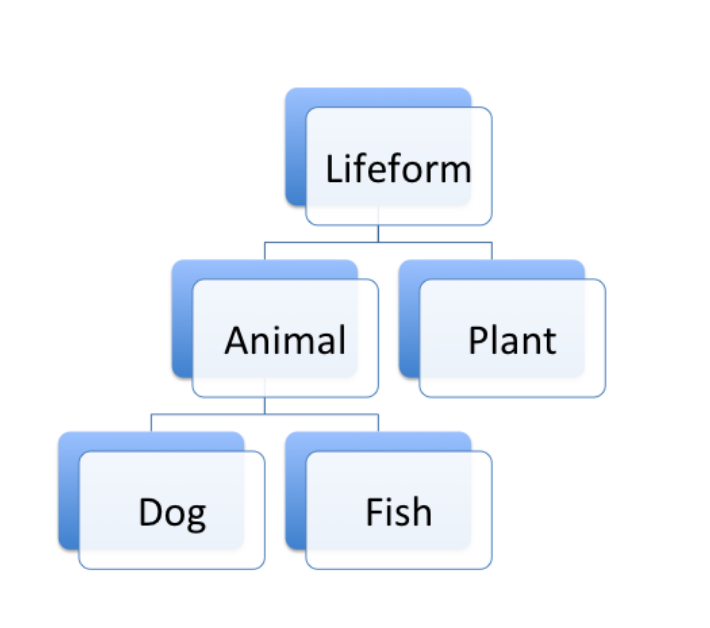
\includegraphics[height=7cm, keepaspectratio]{images/inheritance5}
\end{center}
\end{frame}

\begin{frame}[fragile]
\begin{itemize}
\item Animal interface
\end{itemize}
\begin{block}{}
\begin{lstlisting}
interface Animal{
   public static final int CONSTANT_VARIABLE = 42;
   
   String makeSound();

}
\end{lstlisting}
\end{block}
\end{frame}

\begin{frame}[fragile]
\begin{itemize}
\item Classes implement an interface 
\end{itemize}
\begin{block}{}
\begin{lstlisting}

public class Fox implements Animal{
    public String makeSound(){
    	return "Ring-ding-ding-ding-dingeringeding!";
    }
}
\end{lstlisting}
\end{block}
\end{frame}

\begin{frame}
\begin{itemize}
\item Important to note that Interfaces are not classes
\item ... they can not be instantiated 
\item ... they cannot share a name with a class
\item ... cannot contain implemented methods 
\item ... can only contain method stubs and constants
\end{itemize}
\end{frame}

\begin{frame}
\begin{itemize}
\item Interfaces are more properly described as \textbf{design patterns}
\item They are, therefore, free of some of the restrictions applied to classes
\item You can, for example implement two interfaces in a single subclass
\end{itemize}
\end{frame}

\begin{frame}[fragile]
\begin{block}{}
\begin{lstlisting}
public class Fox implements Lifeform, Animal{
    ...
}

public class Tree implements Lifeform, Plant{
    ...
}
\end{lstlisting}
\end{block}
\end{frame}

\begin{frame}
\begin{center}
\textbf{Aside : Multiple Inheritance}
\end{center}
\begin{itemize}
\item This is the closest that Java comes to allowing two superclasses (parents) in an inheritance heirarchy
\bigskip
\item Subclasses can extend a superclass and implement one or more interfaces
\item Or simply implement one or more interfaces
\end{itemize}
\end{frame}

\begin{frame}
\begin{center}
\textbf{Aside : Multiple Inheritance}
\end{center}
\begin{itemize}
\item Having a class inherit directly from multiple ancestors.
\item Each object oriented programming language has its own rules.
\item Java forbids it for classes.
\item Java permits it for interfaces.
\bigskip
\item Why? (answer later on...)
\end{itemize}
\end{frame}

\begin{frame}[fragile]
\begin{center}
\textbf{Back to Interfaces}
\end{center}
\begin{itemize}
\item Classes implementing an Interface do not inherit code, but ...
\item ... are subtypes of the interface type.
\item So, polymorphism is available with interfaces as well as classes.
\end{itemize}
\begin{block}{}
\begin{lstlisting}
Animal fox = new Fox();

Item item = new CD();
Item item = new Video();
\end{lstlisting}
\end{block}
\end{frame}

\begin{frame}
\begin{center}
\textbf{Bringing this all together...}
\end{center}
\begin{itemize}
\item Interfaces should be used if you
\bigskip
\item Know what to do but don't know how to do it
\item Expect unrelated classes to implement your interface
\item Want to specify the behaviour of a particular data type...
\item ... but are not concerned about who implements its behaviour
\item You want to take advantage of multiple inheritance of type
\end{itemize}
\end{frame}

\begin{frame}
\begin{center}
\textbf{Bringing this all together...}
\end{center}
\begin{itemize}
\item For example, 
\bigskip
\item ... consider methods of payment accepted in your application
\item ... we know we need to take payment but there are different ways of paying
\item ... e.g. Credit Card, PayPal etc..
\end{itemize}
\end{frame}

\begin{frame}[fragile]
\begin{block}{}
\begin{lstlisting}
interface Payment{
    void makePayment(double debit);
}
\end{lstlisting}
\end{block}
\end{frame}

\begin{frame}[fragile]
\begin{block}{}
\begin{lstlisting}
public class PayPal implements Payment{
    public void makePayment(double debit) {
        // logic for PayPal payment
        // e.g. Paypal uses username and password for payment
    }
}
public class CreditCard implements Payment{
    public void makePayment(double debit){
        // logic for CreditCard payment
        // e.g. CreditCard uses card number, date of expiry etc...
    }
}
\end{lstlisting}
\end{block}
\end{frame}

\begin{frame}[fragile]
\begin{block}{}
\begin{lstlisting}
public class NozamaUserDetails{
    
    private String name;
    private Payment paymentMethod;
    
    public NozamaUserDetails(String name, Payment paymentMethod){
    	this.name = name;
	this.paymentMethod = paymentMethod;
    }
    
    // other methods...
}
\end{lstlisting}
\end{block}
\end{frame}

\begin{frame}[fragile]
\begin{block}{}
\begin{lstlisting}
public class NozamaRegisterUser{
    
   public NozamaUserDetails registerUser(String name){
        Payment p = getPaymentMethod();
        return new NozamaUserDetails(name, paymentMethod);
    }
    
    private Payment getPaymentMethod(){
    	return new PayPal();
    }
}
\end{lstlisting}
\end{block}
\end{frame}

\begin{frame}[fragile]
\begin{block}{}
\begin{lstlisting}
public class ProcessPayment{
       
    public void purchase(NozamaUserDetails user, Item item){
    	Payment p = user.getPaymentMethod();
	p.makePayment(item.getPrice());
    }
    
    // other methods...
}
\end{lstlisting}
\end{block}
\end{frame}

% *** ABSTRACT CLASSES ***
\begin{frame}
\begin{center}
\textbf{Abstract Classes}
\end{center}
\end{frame}

\begin{frame}
\begin{center}
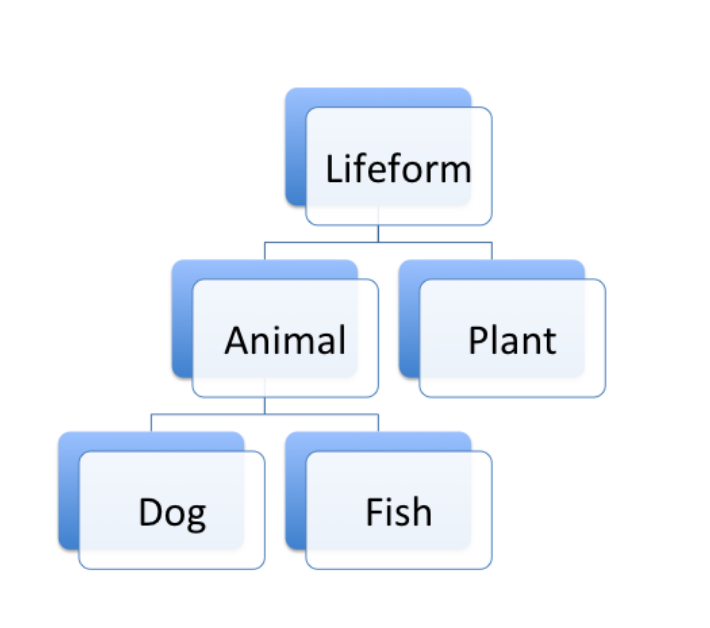
\includegraphics[height=7cm, keepaspectratio]{images/inheritance5}
\end{center}
\end{frame}

\begin{frame}
\begin{itemize}
\item In some situations, however, we may want to include methods in superclasses but only allow them to be used by subclasses
\item For example, in the Animal class we might want to include common functionality for all animals 
\item ... such as average life span
\end{itemize}
\end{frame}

\begin{frame}[fragile]
\begin{itemize}
\item ... we may also want to include an makeSound() method in the Animal class 
\item ... but only allow it to be used in classes that describe specific kinds of animal (i.e. in subclasses of Animal)
\bigskip
\item In these cases, we can use abstract classes and methods
\end{itemize}
\end{frame}

\begin{frame}[fragile]
\begin{block}{}
\begin{lstlisting}
public abstract class Animal{
   private int averageAge;
   
   public Animal(int averageAge){
       this.averageAge = averageAge;
   }

   public int getAverageAge(){
      return averageAge;
   }
   
   // more methods 
   
   // Make the sound of this animal
   abstract void makeSound();  
}
\end{lstlisting}
\end{block}
\end{frame}

\begin{frame}[fragile]
\begin{block}{}
\begin{lstlisting}
public class Dog extends Animal{

   private String sound;
   
   public Dog(int averageAge, String sound){
       super(averageAge);
       this.sound = sound;
   }
   
   // Make the sound of this animal
   public void makeSound(){
       System.out.println("The dog goes " + sound);
   }  
}
\end{lstlisting}
\end{block}
\end{frame}

\begin{frame}
\begin{itemize}
\item Abstract methods have abstract in the signature
\item Abstract methods have no body
\item Abstract methods make the class abstract
\item \textbf{Abstract classes cannot be instantiated}
\item Concrete subclasses complete the implementation
\end{itemize}
\end{frame}

\begin{frame}
\begin{itemize}
\item Note that some methods can still be written in full in an abstract class \ ('implemented{}' methods)
\bigskip
\item So an abstract class can have 
\begin{itemize}
\item constants
\item fields
\item abstract methods
\item implemented methods
\end{itemize}
\end{itemize}
\end{frame}

\begin{frame}
\begin{itemize}
\item Also note that, like Interfaces, Abstract Classes can not be instantiated
\item Classes implementing an Abstract Class are subtypes of the Abstract Class type.
\item So, polymorphism is available with Abstract Class as well as classes.
\end{itemize}
\end{frame}

\begin{frame}
\begin{center}
\textbf{Bringing this all together...}
\end{center}
\begin{itemize}
\item For example, 
\bigskip
\item ... consider methods of payment accepted in your application
\item ... we know we need to take payment but there are different ways of paying
\item ... e.g. Credit Card, PayPal etc..
\end{itemize}
\end{frame}

\begin{frame}
\begin{center}
\textbf{Bringing this all together...}
\end{center}
\begin{itemize}
\item BUT, if for example... 
\item ... each payment type (PayPal, Credit Card etc.) needs to be authorised by a Bank
\item ... and this process is the same for all types of payment
\item ... and we don't want programmers to reimplement this each time
\bigskip
\item ... we would use an Abstract Class to implement this method
\item ... but ensure that programmers implement the makePayment method
\item ... because this is specific to each payment type
\end{itemize}
\end{frame}

\begin{frame}[fragile]
\begin{block}{}
\begin{lstlisting}
public abstract class Payment{

    protected boolean authoriseWithBank(String userAuthKey){
        // logic to authorise payment with bank
    }

    abstract void makePayment(double debit);
}
\end{lstlisting}
\end{block}
\end{frame}

\begin{frame}[fragile]
\begin{block}{}
\begin{lstlisting}
public class PayPal extends Payment{
    public void makePayment(double debit) {
        // logic for PayPal payment
        // e.g. Paypal uses username and password for payment
        super.authoriseWithBank(authToken);
    }
}
public class CreditCard extends Payment{
    public void makePayment(double debit){
        // logic for CreditCard payment
        // e.g. CreditCard uses card number, date of expiry etc...
        super.authoriseWithBank(authToken);
    }
}
\end{lstlisting}
\end{block}
\end{frame}

\begin{frame}[fragile]
\begin{block}{}
\begin{lstlisting}
public class NozamaUserDetails{
    
    private String name;
    private Payment paymentMethod;
    
    public NozamaUserDetails(String name, Payment paymentMethod){
    	this.name = name;
	this.paymentMethod = paymentMethod;
    }
    
    // other methods...
}
\end{lstlisting}
\end{block}
\end{frame}

\begin{frame}[fragile]
\begin{block}{}
\begin{lstlisting}
public class NozamaRegisterUser{
    
   public NozamaUserDetails registerUser(String name){
        Payment p = getPaymentMethod();
        return new NozamaUserDetails(name, paymentMethod);
    }
    
    private Payment getPaymentMethod(){
    	return new PayPal();
    }
}
\end{lstlisting}
\end{block}
\end{frame}

\begin{frame}[fragile]
\begin{block}{}
\begin{lstlisting}
public class ProcessPayment{
       
    public void purchase(NozamaUserDetails user, Item item){
    	Payment p = user.getPaymentMethod();
	p.makePayment(item.getPrice());
    }
    
    // other methods...
}
\end{lstlisting}
\end{block}
\end{frame}

\begin{frame}
\begin{itemize}
\item Abstract classes should be used if you
\bigskip
\item Want to share code among several closely related classes
\item Expect that classes that extend your abstract class have many common methods or  fields, or require access modifiers other than public (such as protected and private)
\item Want to declare non-static or non- final fields (interfaces).  This enables you to define methods that can access and modify the state of the object to which they belong
\end{itemize}
\end{frame}

%*** Multiple Inheritance ANSWER HERE !!!! ****
\begin{frame}
%\begin{center}
%\textbf{Aside : Multiple Inheritance}
%\end{center}
\begin{itemize}
\item Note, however, that abstract classes are still classes
\item ... more specifically, partially implemented classes
\bigskip
\item So the rules that govern implemented classes also govern abstract classes 
\item i.e. no subclass can have two (or more) abstract parents
\end{itemize}
\end{frame}

\begin{frame}
\begin{center}
\textbf{Aside : Multiple Inheritance}
\end{center}
\begin{itemize}
\item Having a class inherit directly from multiple ancestors.
\item Each object oriented programming language has its own rules.
\item Java forbids it for classes.
\item Java permits it for interfaces.
\bigskip
\item Why? (answer later on...)
\end{itemize}
\end{frame}

\begin{frame}
\begin{center}
\textbf{Aside : Multiple Inheritance}
\end{center}
\begin{itemize}
\item Answer is - avoids competing definitions of methods or fields?
\end{itemize}
\end{frame}

\begin{frame}
\begin{center}
\textbf{Dimond Problem}
\end{center}
\begin{center}
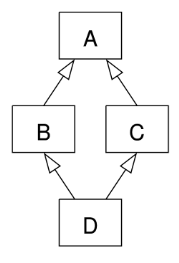
\includegraphics[height=6cm, keepaspectratio]{images/diamond}
\end{center}
\end{frame}

\begin{frame}
\begin{center}
\textbf{Dimond Problem}
\end{center}
\begin{columns}
\begin{column}{0.6\textwidth}
\begin{itemize}
\item Two classes B and C
\item ... inherit from A
\end{itemize}
\end{column}
\begin{column}{0.4\textwidth}
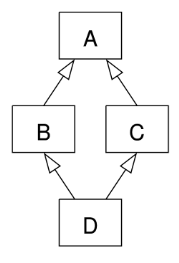
\includegraphics[height=6cm, keepaspectratio]{images/diamond}
\end{column}
\end{columns}
\end{frame}

\begin{frame}
\begin{center}
\textbf{Aside : Multiple Inheritance}
\end{center}
\begin{columns}
\begin{column}{0.6\textwidth}
\begin{itemize}
\item ... another class D 
\item ... inherits from both B and C
\end{itemize}
\end{column}
\begin{column}{0.4\textwidth}
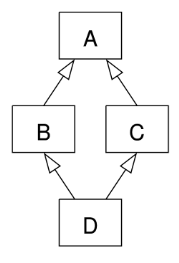
\includegraphics[height=6cm, keepaspectratio]{images/diamond}
\end{column}
\end{columns}
\end{frame}

\begin{frame}
\begin{center}
\textbf{Aside : Multiple Inheritance}
\end{center}
\begin{columns}
\begin{column}{0.6\textwidth}
\begin{itemize}
\item If there is a method in A 
\item ... that B and/or C has overridden
\item ... and D does not override it
\bigskip
\item Then which version of the method does D inherit? 
\item ... that of B, or that of C?
\end{itemize}
\end{column}
\begin{column}{0.4\textwidth}
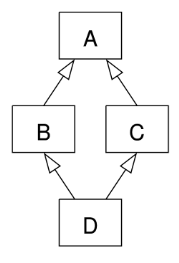
\includegraphics[height=6cm, keepaspectratio]{images/diamond}
\end{column}
\end{columns}
\end{frame}

\begin{frame}[fragile]
\begin{center}
\textbf{Aside : Multiple Inheritance}
\end{center}
\begin{block}{}
\begin{lstlisting}
public class Book {
    public void getContent(){
        return content;
    }
}
\end{lstlisting}
\end{block}
\end{frame}

\begin{frame}[fragile]
\begin{center}
\textbf{Aside : Multiple Inheritance}
\end{center}
\begin{block}{}
\begin{lstlisting}
public class AudioBook extends Book{
    public void getContent(){
        return audioContent;
    }
}


public class EBook extends Book { 
    public void getContent(){
        return ebookContent;
    }
 }
\end{lstlisting}
\end{block}
\end{frame}

\begin{frame}[fragile]
\begin{center}
\textbf{Aside : Multiple Inheritance}
\end{center}
\begin{block}{}
\begin{lstlisting}
public class MultiMediaBook extends AudioBook, EBook{
    
    // other methods BUT NOT getContent()!
    
    public static void main(String[] args){
        MultiMediaBook mmb = new MultiMediaBook();
        mmb.getContent();
        // which getContent do we use?
        // AudioBook or EBook?
    }
}
\end{lstlisting}
\end{block}
\end{frame}

\begin{frame}
\begin{center}
\textbf{Aside : Multiple Inheritance}
\end{center}
\begin{itemize}
\item Java forbids it for classes.
\item Java permits it for interfaces.
\item So, there are no competing implementations.
\bigskip
\item For interest:  Java 8 introduces default methods for interfaces which can lead to the diamond problem
\item Therefore, the Java compiler provides rules to determine which default method a particular class uses
\end{itemize}
\end{frame}

% *** Choosing An Interface or Abstract Class
\begin{frame}
\begin{center}
\textbf{Interfaces vs Abstract Classes}
\end{center}
\begin{itemize}
\item It can be difficult to identify 
\begin{itemize}
\item when to use an abstract class
\item when to use an interface
\end{itemize}
\item As a simple rule of thumb, when faced with a choice between abstract classes and interfaces
\begin{itemize}
\item use an abstract class when
\item you want to implement some but not all of a class's methods
\item and you are willing to accept the restrictions imposed upon classes
\item e.g. single inheritance
\item otherwise use an interface
\end{itemize}
\end{itemize}
\end{frame}

% *** Finally ***
%\begin{frame}
%\begin{center}
%\textbf{Finally...}
%\end{center}
%\end{frame}
%
%\begin{frame}
%\begin{itemize}
%\item Finally (for now) note that abstract superclasses can have abstract subclasses 
%\item If, for some reason we don't want to implement all the methods in an abstract superclass (parent), we can
%\begin{itemize}
%\item implement some methods
%\item leave other methods as abstract
%\item and declare the subclass (child) as abstract
%\end{itemize}
%\item This approach will leave the subclass's subclasses to instantiate the other abstract methods (or their subclasses,
%subclass's subclasses etc.)
%\end{itemize}
%\end{frame}
%
%\begin{frame}[fragile]
%\begin{itemize}
%\item Abstract classes can also implement interfaces
%\end{itemize}
%\begin{block}{}
%\begin{lstlisting}
%abstract class Canine implements Animal { 
%	...
%}
%\end{lstlisting}
%\end{block}
%\end{frame}
%
%\begin{frame}[fragile]
%\begin{itemize}
%\item Similarly, Interfaces can also extend other interfaces
%\end{itemize}
%\begin{block}{}
%\begin{lstlisting}
%interface Animal extends Lifeform{
%...
%}
%
%interface Dog extends Animal, Lifeform{
%...
%}
%\end{lstlisting}
%\end{block}
%\end{frame}


% *** HERE ***
\begin{frame}
\begin{center}
\textbf{Summary}
\end{center}
\begin{itemize}
\item Inheritance can provide shared implementation...
\item ... both as concrete and abstract classes
\item Inheritance provides shared type information
\item ... interfaces
\end{itemize}
\end{frame}

\begin{frame}
\begin{center}
\textbf{Summary}
\end{center}
\begin{itemize}
\item Abstract classes function as incomplete superclasses
\item Interfaces provide specification without implementation
\bigskip
\item Both Interfaces and Abstract Classes support polymorphism
\end{itemize}
\end{frame}

\end{document}